\graphicspath{{Chapters/TGCLimits/Figures/}}
\chapter{Limits on Anomalous Neutral Triple Gauge Couplings}
\label{chap:TGCLimits}

\section{Limit Setting Procedure}

\subsection{Matrix Element Reweighting}
As described in~\sec{TheoryZZ-TGCs}, anomalous neutral triple gauge couplings affecting \ZZ\
production are described by four parameters, \ffourg, \ffourZ, \ffiveg\ and
\ffiveZ.
Since the parameters enter linearly in the effective Lagrangian
(\eqn{tgc-lagrangian}), they will appear
quadratically in the amplitude of the \ZZllll\ process. The differential \cx\
can thus be written as:
\begin{eqnarray}\label{eqn:dsigma}
{\rm d}\sigma_{\rm SM+TGC} & = & F_{00} + f_4^\gamma F_{01} + f_4^Z F_{02} + f_5^\gamma F_{03} + f_5^Z F_{04}  \nonumber \\
&+& \left(f_4^\gamma\right)^2F_{11} + f_4^\gamma f_4^Z F_{12} +  f_4^\gamma f_5^\gamma F_{13} + f_4^\gamma f_5^Z F_{14}  \nonumber \\
&+& \left(f_4^Z\right)^2F_{22} + f_4^Zf_5^\gamma F_{23} + f_4^Zf_5^Z F_{24}  \nonumber \\
&+& \left(f_5^\gamma\right)^2F_{33} + f_5^\gamma f_5^Z F_{34} \nonumber \\
&+& \left(f_5^Z\right)^2F_{44}
\end{eqnarray}
where $F_{ij}$ are coefficients describing how the \cx\ changes in the presence
of \TGC s. A priori, there are 25 coefficients, however, using the 
symmetry property of the coefficients ($F_{ij}=F_{ji}$), it is seen 
that only $25-10=15$ are independent. $F_{00}$ corresponds to the contribution
of the \sm\ diagrams and the rest consist of operator contributions associated with the
anomalous couplings. 

A simulated event generated assuming only \sm\ couplings can be assigned a weight corresponding to the differential \cx\
assuming \TGC\ couplings at some specific value of the four parameters:
\begin{equation}
{\rm weight} = \frac{{\rm d}\sigma_{\rm SM+TGC}(\ffourg, \ffourZ, \ffiveg,
\ffiveZ)}{{\rm d}\sigma_{\rm SM}}
\end{equation}
By assigning such a weight to every event in the sample, it is possible to reweight a sample
generated with only \sm\ couplings to a sample with \TGC\ couplings.
This procedure can be easily extended to reweight a sample generated assuming
any given set of \TGC s to any other set of \TGC s. For example, to reweight a sample
generated assuming only \sm\ couplings to sample assuming \ffourg=0.1, one would
apply to each event a weight:
\begin{eqnarray}\label{revisit}
{\rm weight} = \frac{F_{00} + 0.1 \cdot  F_{01} + (0.1)^{2} \cdot
F_{11}}{F_{00}}
\end{eqnarray}
The \Fij\ coefficients are completely
specified by the kinematics of the incoming and outgoing particles, and so must
be evaluated on an event by event basis. They are
independent of the values of the anomalous coupling parameters, although they do depend on
the choice of \formfactor. The coefficients are determined using matrix elements for
\ZZllll\ production in the presence of \TGC s, as follows. By using Equation~\ref{eqn:dsigma} it 
is possible to write down 15 equations that uniquely determine the 
coefficients $F_{ij}$ in terms of matrix elements assuming particular values
for the \TGC\ couplings.
To illustrate the procedure, consider the simplified situation where 
there is just one coupling constant $f$. In this case, there are 3 coefficients 
to be determined:
\begin{eqnarray}\label{revisit2}
{\rm d}\sigma_{\rm SM+TGC} = F_0 + fF_1 + f^2F_2 
\end{eqnarray}
where  $F_0={\rm d}\sigma_{\rm SM}$.

Using three different values of $f$, e.g $f=\{0,1,-1\}$, three independent
equations may be written down:
\begin{eqnarray}\label{matrix1}
\left(\begin{array}{c}
{\rm d}\sigma_1\\
{\rm d}\sigma_2\\
{\rm d}\sigma_3
\end{array}\right) =
\left[\begin{array}{ccc}
1 & 0 & 0 \\
1 & 1 & 1 \\
1 & -1 & 1
\end{array}\right]
\left(\begin{array}{c}
F_0\\
F_1\\
F_2
\end{array}\right)
\end{eqnarray}
Denoting the matrix containing the coupling values $\hat{A}$, the cross sections
\dsigmavec\ and the coefficients $\vec{F}$, the equations are easily
manipulated to give the coefficients 
\begin{eqnarray}\label{matrix2} \dsigmavec=\hat{A}\vec{F} \qquad \Rightarrow \qquad \vec{F}=\hat{A}^{-1}{\rm
\bf d}\vec{\sigma} 
\end{eqnarray} 
This requires that $\hat{A}$ must be invertible. This is the
case if the couplings are chosen such that the three equations in~\ref{matrix1}
are independent. When considering all four couplings at the same time, the
matrix $\hat{A}$ is 15$\times$15 and \dsigmavec\ and $\vec{F}$ are
15-dimensional vectors.

The \TGC\ matrix elements are obtained from the next-to-leading order \mc\
generator \BHO~\cite{bho}. Matrix elements from the leading-order \BR\
generator~\cite{Baur:1994au} are also used as a cross-check. The matrix
elements are introduced into the  framework described in~\cite{Bella:2008wc},
which enables a calculation of the amplitude given the four-vectors and PDG
codes of the incoming partons and outgoing particles from the hard process. 

Whilst it is possible to reweight a \sm\ sample to a \TGC\ point, this suffers
from a lack of statistics in the tails of distributions such as the \Z\ boson \pt\ 
and the four-lepton invariant mass, where the presence of \TGC s
enhances the cross section at high momentum and high invariant mass. Instead,
samples generated with values of the \TGC\ couplings set near previously set
experimental limits are used; this ensures statistics in the tails of the
distributions of interest. The \powhegbox\ and \ggZZ\ generators used to generate the nominal signal
samples do not model \TGC s; instead the samples are generated using \sherpa,
which does. For the 7~\tev\ analysis, four samples are used, with couplings
 $\{f_{4}^{\gamma}=0.1\}$, $\{f_{5}^{\gamma}=-0.1\}$,
$\{f_{4}^{\gamma}=0.1$ \& $f_{5}^{\gamma}=0.1\}$, and 
$\{f_{4}^{Z}=0.1$ \& $f_5^{Z}=0.1\}$. For the 8~\tev\ analysis, three sample are
used, with couplings $\ffourgamma=0.1\}\}$ (denoted TGC0),
$\{\ffourgamma=0.1 \& \ffiveZ=0.1\}$ (denoted TGC1), and 
$\{ \ffourgamma = \ffourZ = \ffivegamma = \ffiveZ \}$ (denoted TGC2). The 7~\tev\ samples are
generated with a \formfactor of $\Lambda=2\tev,n=3$; the 8~\tev\ samples are
generated without a \formfactor. The reweighting procedure can of course be used to
reweight samples generated with one \formfactor (or no \formfactor) to another
\formfactor.

\subsection{Validation of Reweighting Procedure}

To demonstrate the performance of the reweighting procedure, the 8~\tev\ \sherpa\
samples generated with \TGC s are reweighted to the \sm\ (i.e. no \TGC s), and
compared to a sample generated with only \sm\ couplings, and the TGC1 and TGC2
samples were reweighted to the TGC0 sample. \fig{} shows the
resulting distributions of the \pt\ of the leading \Z\ boson, and the ratios of
the reweighted samples to the \sm/TGC0 distribution for reweighting carried out
using the \BHO\ and \BR\ matrix elements. For both the generators, the reweighted samples are seen
to agree well with the directly generated sample.

\begin{figure}[htbp]
\begin{center}
\subfigure[]{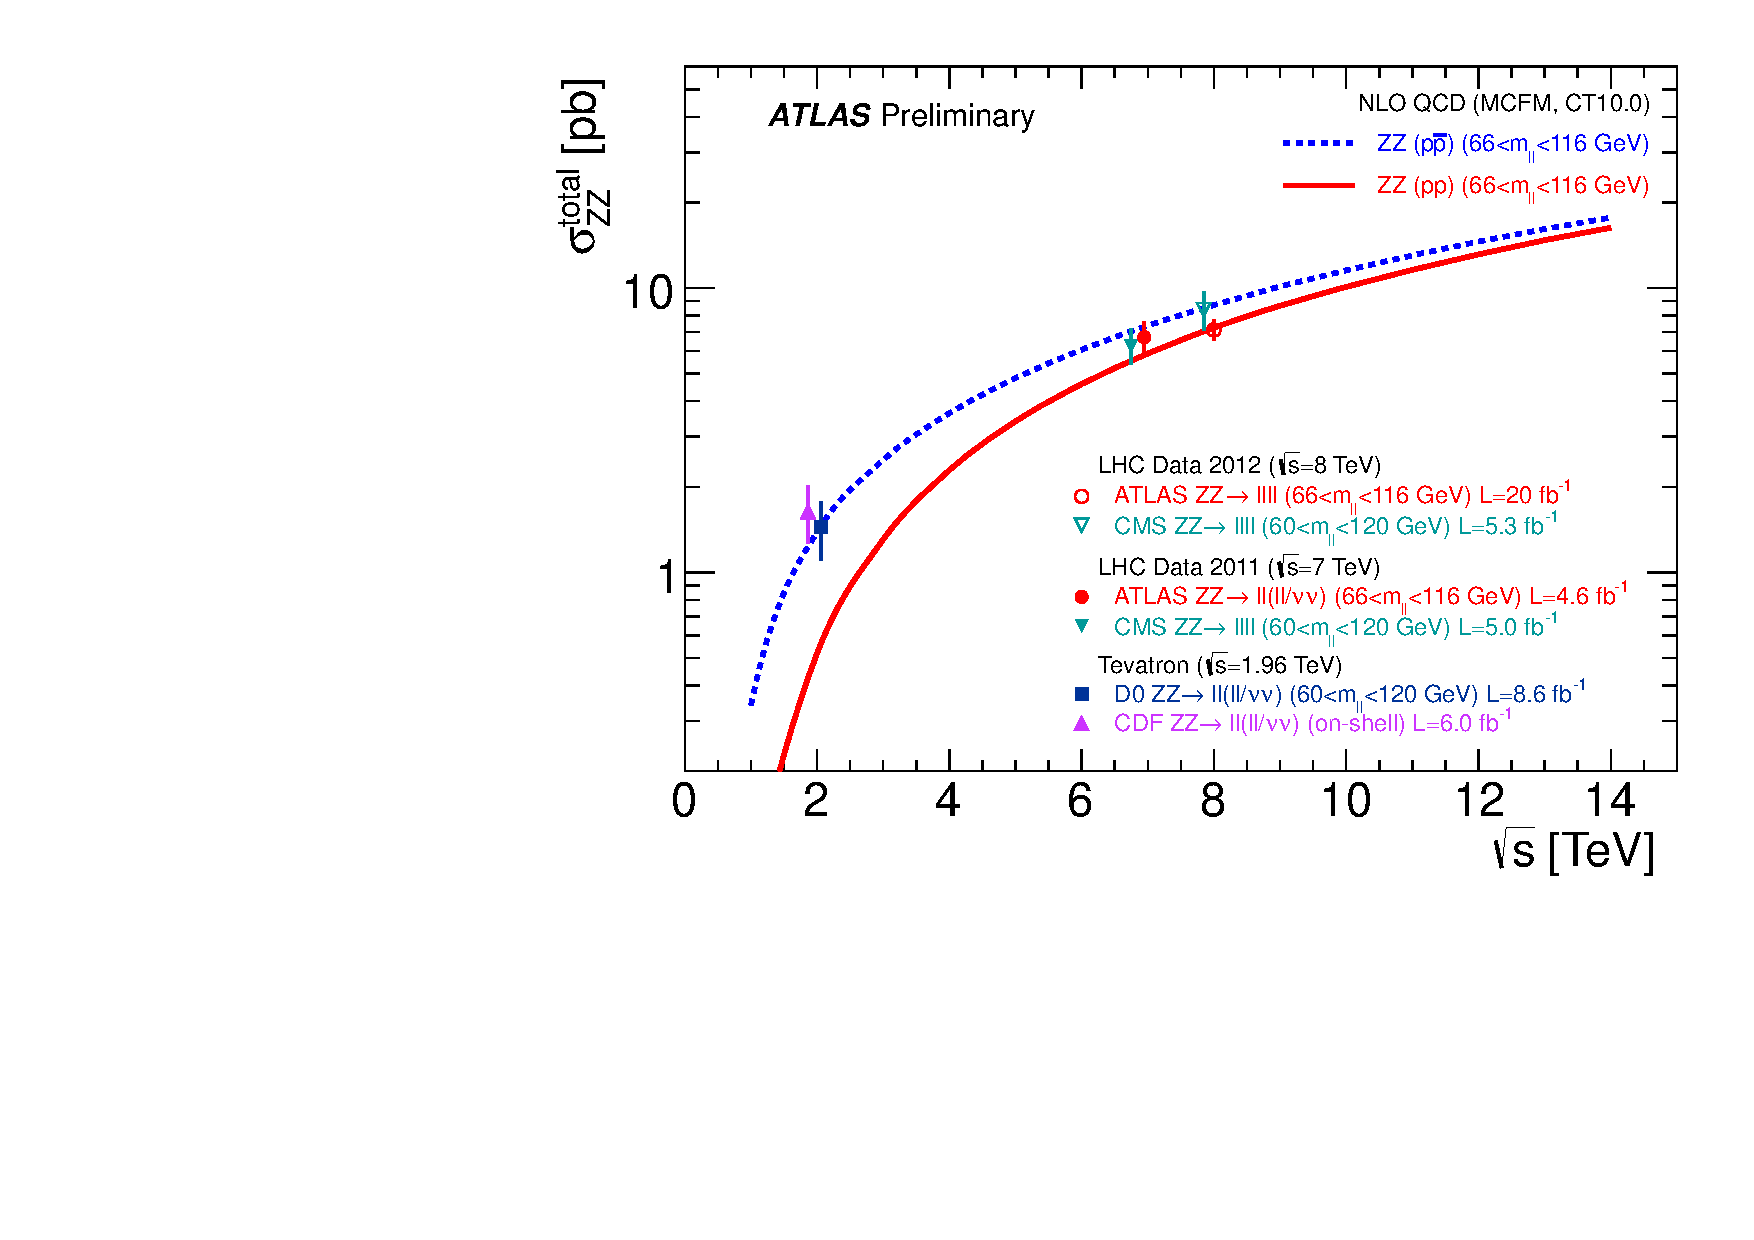
\includegraphics[width=0.9\textwidth]{SigmaZZatNLO}}
\caption{
\small
Comparison of experimental measurements and theoretical predictions of the total
\ZZ\ production \cx\ as a function of centre-of-mass energy $\sqrt{s}$. Shown
are experimental measurements from CDF~\cite{CDF:2011ab} and
D0~\cite{Abazov:2012cj} in $p\bar{p}$ collisions at the Tevatron at $\sqrt{s} =
1.96$~TeV, and experimental measurements from ATLAS~\cite{ATLAS:2012kg} and
CMS~\cite{CMS:2012rg,CMS:2013oev} in $pp$ collisions at the LHC at $\sqrt{s} =
7$~TeV and $\sqrt{s} = 8$~TeV. The blue dashed line shows the theoretical
prediction for the \ZZ\ production cross section in $p\bar{p}$ collisions,
calculated at NLO in QCD using MCFM with PDF set CT10. The solid red line shows
the theoretical prediction for the \ZZ\ production cross section in $pp$
collisions, calculated in the same way.  The theoretical curves are calculated
using the natural width of the $Z$ boson in the mass range 66 to 116 GeV.
 %At $\sqrt{s}=8$ TeV, the theoretical prediction using the zero-width
 %approximation is 5\% higher than the prediction using the natural width,
 %restricted to the mass range 66 to 116 GeV.
 }
\label{fig:sqrts-plot}
\end{center}
\end{figure}

\subsection{Yield Coefficients}

In order to extract limits on the \TGC s, the number of expected events as a
function of the \TGC\ couplings must be predicted. This is parameterised by
yield coefficients \Yij, which may be obtained from the \Fij\ as:
\begin{equation}
\Yij = \left( \sum_{\rm events} \frac{F_{ij}}{F_{00} } \right) \cdot{N_{\rm expected}}.
\end{equation}
where $N_{\rm expected}$ is the \sm\ number of expected events obtained from the
nominal signal sample and the sum is over events passing the full event
selection. Event level lepton efficiency, energy scale, and resolution corrections
are taken into account when calculating the yield coefficients. A different set of yield
coefficients is needed for each bin of the differential distribution used to set
the limits, and different yield coefficients are needed for each choice of
form-factor. 

\tab{yield-coeff-seven} shows the yield coefficients for the 7~\tev\ analysis for the
unbinned case with a \formfactor\ of $\Lambda=3~\tev, n=3$ and for the case of
no \formfactor.\tab{yield-coeff-eight} shows the coefficients for the 8~\tev\
analysis. The yield coefficients for each bin of the differential distributions
are shown in Appendix~\ref{appendix:tgc-coeff}.

\subsection{Limit Setting}

The 95\% confidence level (CL) intervals for the \TGC\ parameters are determined
using a frequentist maximum profile-likelihood based method~\cite{Cowan:2010js}.
%on the number of observed events in each bin
%of the differential distributions, with systematic uncertainties introduced as
%nuisance parameters. 
The three \lllplp\ final states are each merged prior to
the profile-likelihood maximisation. The likelihood function is similar
to that used in the cross section calculation, but parametrised in terms of the
number of events in each bin instead of the \cx.  Nuisance parameters are
again represented with Gaussian terms ($G$); since there are nuisance
parameters for both signal and background, the set of nuisance parameters giving
the fractional uncertainty on the signal and background expectation for a
distribution of $m$ bins are expressed as:
$\vec\beta = \{\beta_1, \beta_2, \ldots, \beta_{2m}\}$, where:
\begin{eqnarray}
\text{true }N_\mathrm{sig}^i &=& N_\mathrm{sig}^i \cdot (1 + \beta_i) \label{nuis1}\\
\text{true }N_\mathrm{bkg}^i &=& N_\mathrm{bkg}^i \cdot (1 + \beta_{i+m}) \label{nuis2}
\end{eqnarray}
The likelihood function is then given as:
\begin{equation}
L(\vec{f}, \vec{\beta}) =
\prod_{i=1}^{m}P(N_\mathrm{data}^i,\mu^i(\vec{f},\vec\beta))
\times
\frac{1}{(2\pi)^m}e^{-\frac{1}{2}\left(\vec\beta\cdot C^{-1}\cdot\vec\beta\right)},
\label{likelihood}
\end{equation}
where $\vec{f}=\{\ffourg, \ffourZ, \ffiveg, \ffiveZ \}$ are the \TGC\
parameters and $\mu^{i}$ is the expected number of events in bin $i$:
\begin{equation}
\mu^i(\vec{f},\vec{\beta})
= N_\mathrm{sig}^i(\vec{f})(1 + \beta_i) + N_\mathrm{bkg}^i(1 + \beta_{i+m}).
\end{equation}
with:
\begin{equation}
N_{\rm sig} = (Y_\mathrm{\rm SM} + Y_{f_i^V}\cdot f_i^V + Y_{f_i^Vf_i^V}\cdot (f_i^V)^2)\cdot\mathcal{L}\cdot{C_{ZZ}}.
\end{equation}

A test statistic \teststat\ is constructed as the ratio of the \maxprofilellh\
at a test value of the \TGC\ parameters $\vec{f}$ to the full \maxprofilellh:
\begin{equation}
\teststat =
\frac{L(N|\vec{f},\vec{\hat{\hat{\beta}}})}{L(N|\vec{\hat{f}},\vec{\hat{\beta}})}
\end{equation}
where $\vec{\betahathat}$ is the value of $\vec{\beta}$ that maximises the
numerator, and $\vec{\hat{f}}$ and $\vec{\hat{\beta}}$ are the values of
$\vec{f}$ and $\vec{\beta}$ that maximise the numerator. The distribution of
\teststat\ in the assumption of \TGC\ couplings at the test value of the
parameters is obtained by generating 10,000 pseudo experiments. In each
pseudo experiment the nuisance parameters $\vec{\beta}$ are Gaussian
fluctuated around the mean value of $\vec{\betahathat}$ and the number of events
$N_{PE}$ are drawn randomly from a Poisson distribution with a mean corresponding to the
values of $\vec{f}$ and $\vec{\beta}$. The $p$-value at the test value of the
couplings is calculated as the fraction of pseudo-experiments which have a test
statistic smaller than the observed value of the test statistic $\teststat_{obs}$.
This procedure is repeated scanning values of $\vec{f}$, and the 95 \%
confidence interval is define by all values of $\vec{f}$ for which
$p(\vec{f})\geq 5\%$. Limits are set for one \TGC\ parameter at a time, holding
the other parameter at their \sm\ values of zero. The expected sensitivity is
also obtained using pseudo-experiments. In each
experiment, $N^{i}_{sig}$ and $N^{i}_{bg}$ are given by the \sm\ expectations but
allowed to fluctuate within their uncertainties.

\section{Bin Optimisation}

For the 7~\tev\ analysis, limits were set using the total number of observed
events, and by using the number of events observed in bins of the leading \Z\
boson \pt\ and in bins of the mass of the four-lepton system. 

Binning for 7~\tev\ analysis?

For the 8~\tev\ analysis, a bin optimisation procedure was carried out, varying
the number of bins, and the bin boundaries. For each variation, a set of XX
pseudo-experiments is carried out in order to derive the expected limit. For
each binning considered, the systematic uncertainties on the expected \sm\ signal
in each bin are re-evaluated, as well the theoretical uncertainties on the
differential \cx. The estimated irreducible background is re-derived from the
\mc. The irreducible background per bin is obtained by dividing the total
data-driven estimate according to the background shape obtained from data. The
fractional systematic and statistical uncertainty on the data-drive background
estimate is assumed to be the same in every bin. No systematic to
account for uncertainties on the reducible background shape is assigned. This
approach is justified by the fact that the total background uncertainty is
already large, and that the background contribution above XX is very small.
This procedure means that large statistical uncertainties on the expected \sm\
signal and large PDF and scale errors when the last bin boundary is very high are taken into account. It does
not however take into account that there may be large statistical errors
associated with the estimate of the reconstruction systematic uncertainties when
there are limited statistics in the \sm\ \mc\ sample in the last bin. Therefore
before choosing a final binning it is checked that the statistics in the last
bin are sufficient to properly evaluate the systematics.

\section{Expected Limits}

Expected limits for 1 bin, many bins, BR/BHO, different FF

\section{Observed Limits}
